\documentclass{uninove-ppgi} %courier ou times

\begin{document}
\lstset{
    language=xml,
    tabsize=3,
    frame=shadowbox,
    rulesepcolor=\color{gray},
    xleftmargin=20pt,
    framexleftmargin=15pt,
    keywordstyle=\color{blue}\bf,
    commentstyle=\color{OliveGreen},
    stringstyle=\color{red},
    numbers=left,
    numberstyle=\tiny,
    numbersep=5pt,
    breaklines=true,
    showstringspaces=false,
    basicstyle=\footnotesize,
    emph={food,name,price},emphstyle={\color{magenta}}
}

% Posiciona o logo da Uni9 no topo

\includegraphics[height=1.5cm]{uninove-logo}

% parametros de capa e folha de rosto (é necessário configurar todos)
\Universidade{UNIVERSIDADE NOVE DE JULHO - UNINOVE}

\Autor{EXCLUÍDOS OS DADOS SOBRE OS AUTORES EM ATENDIMENTO A LGPD - LEI GERAL DE PROTEÇÃO DE DADOS}

% ATENÇÃO: NÃO INCLUIR NOME E RA DE NENHUM ALUNO
% EM NENHUMA PARTE DO DOCUMENTO

\Titulo{CHAT EM TEMPO REAL}

% Inserir o nome do projeto no formato que está abaixo (Olhe o nome da disciplina na central do aluno)
\Tipoprojeto{PROJETO EM COMPUTAÇÃO APLICADA}

% Informe qual o curso: Bacharel ou Tecnólogo + curso
\Curso{CIÊNCIA DA COMPUTAÇÃO}

% NÃO ALTERAR
\Orientador{Edson Melo de Souza, Dr.}

% Inserir o ano correspondente
\Ano{2024}

% gera a capa automaticamente
\capa

% gera folha de rosto automaticamente
\folharosto

% ##################### Início dos elementos pré-textuais ############################

% Resumo (Obrigatório)
% !TEX root = ..\main.tex

\PalavrasChave{CHAT, JAVASCRIPT, WEBSOCKET, HTML, CSS }
\centeredchapterstyle
\begin{resumo}
    \noindent\textbf{Contexto}:  Chat em tempo real onde a mensagem do usuário será replicada no servidor e encaminhada para todos.
 \textbf{Objetivo}: Comunicar-se em tempo real com qualquer pessoa conectada ao chat.  \textbf{Método}: Usando HTML, CSS e JavaScript para o desenvolvimento front-end e WebSocket para o back-end. \textbf{Resultados}: O usuário pode se comunicar livremente com qualquer pessoa no chat, usando emojis de uma forma muito divertida. \textbf{Conclusão}: Um chat bem prático e divertido
\end{resumo}

% Abstract (Obrigatório) - resumo em inglês
% !TEX root = ..\main.tex

\KeyWords{CHAT, JAVASCRIPT, WEBSOCKET, HTML, CSS}
\centeredchapterstyle
\begin{abstract}
    \noindent\textbf{Contextualization}: Real-time chat where the user's message will be replicated on the server and forwarded to everyone.\textbf{Objetive}:  To communicate in real-time with anyone connected to the chat. \textbf{Method}: Using HTML, CSS, and JavaScript for the front-end development, and WebSocket for the back-end. \textbf{Results}:The user can freely communicate with anyone in the chat, using emojis in a very fun way. \textbf{Conclusion}: A very practical and fun chat.
\end{abstract}


% Sumário (Obrigatório)
\begingroup
\makeatletter \let\ps@plain\ps@empty \makeatother
\tableofcontents % sumário
\endgroup
\thispagestyle{empty}

% Lista de figuras
\renewcommand*\listfigurename{Lista de Ilustrações}
\listoffigures
\thispagestyle{empty}



% ############### Fim dos elementos pré-textuais ######################

\regularchapterstyle

% ############### Início dos Capítulos (Obrigatório ) #################

% Introdução
\chapter{Introdução}
\label{ch:introducao}
\begin{resumocapitulo}
O chat em tempo real funciona exatamente como o nome sugere. O servidor replica todas as mensagens enviadas pelos usuários, sejam elas emojis ou textos.

É um sistema rápido e fácil de usar, onde o usuário apenas insere um nome e pode começar a conversar com outros participantes do chat. O design foi inspirado no aplicativo "WhatsApp", mas de forma mais simplificada. 
\end{resumocapitulo}




% Base Teórica
\chapter{Fundamentação Teórica}
\label{ch:identificador}
	\begin{resumocapitulo}
	 A importância da comunicação 
	\end{resumocapitulo}

	\section{Comunicaçãol}
	O chat foi desenvolvido para facilitar a comunicação em tempo real, permitindo que os usuários façam novas amizades ou conversem com familiares.

Inspirado em aplicações como o WhatsApp, este chat oferece uma experiência simplificada, eliminando a necessidade de verificação via SMS. Basta inserir um nome e começar a conversar imediatamente. Projetado para ser fácil de usar e proporcionar diversão no dia a dia.

	\section{Conteúdo 1}
	\label{sec:identificao}
 O usuário pode inserir um nome, que é automaticamente destacado com uma cor, graças a uma lógica implementada em JavaScript. Isso proporciona uma experiência mais divertida e personalizada. O design é simples e funcional, com o objetivo principal de garantir que as mensagens enviadas no chat sejam claramente visíveis para o usuário.
     

% Metodologia
\chapter{Metodologia}
\label{ch:identificador}
	\begin{resumocapitulo}
		O passo a passo da criação
	\end{resumocapitulo}

	\section{Desenvolvimento}	
Desenvolvemos o backend utilizando JavaScript e WebSocket para proporcionar uma experiência de chat em tempo real.

Inicialmente, implementamos um código que executa e atualiza dinamicamente as funcionalidades à medida que são desenvolvidas. Em seguida, elaboramos toda a estrutura HTML e CSS, começando pela tela inicial. No processo de estilização, o CSS é utilizado para criar uma apresentação visual coesa e atraente.

Por meio do JavaScript, implementamos a lógica necessária para distinguir as mensagens enviadas pelos usuários. Essa lógica garante que as mensagens sejam exibidas à direita quando enviadas pelo usuário local e à esquerda quando provenientes de outros usuários, cada uma com sua própria formatação visual definida previamente no CSS.

	\section{Desenvolvimento}

Durante todo o processo de desenvolvimento, utilizamos o Visual Studio Code , uma plataforma que se destaca pela praticidade e eficiência que oferece.

O design do chat foi meticulosamente planejado para proporcionar uma experiência mais limpa e objetiva aos usuários, através da utilização do modo escuro. Esta abordagem visa promover uma interação mais focada e agradável.

Além disso, o desenvolvimento foi realizado no ambiente Windows 10, com o auxílio da extensão Live Server, uma ferramenta integrada ao Visual Studio Code. O Live Server permite visualizar em tempo real as modificações realizadas no código, facilitando significativamente o processo de desenvolvimento.

 Visual Studio Code - https://code.visualstudio.com/
 

% Resultado
\chapter{Análise dos Resultados}
\label{ch:resultados}


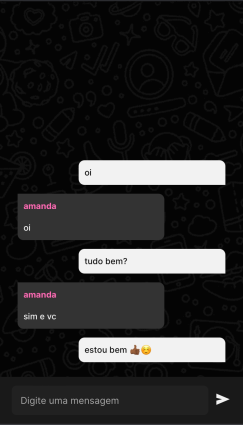
\includegraphics{figuras/mjmb943u.png}






% Conclusão
\chapter{Conclusões}
\label{ch:conclusao}
	O desenvolvimento desta aplicação foi uma experiência gratificante, visando proporcionar aos usuários uma conversa agradável e tranquila, livre de complicações.

Com um design clean e minimalista, nosso chat em tempo real foi projetado para oferecer uma experiência de uso intuitiva e sem distrações, priorizando a comunicação eficaz entre os usuários.



% ##################### Fim dos Capítulos ############################

% Bibliografia (Obrigatório)
\bibliography{refs} Canal Manual do Dev. "Como Criar um Chat em Tempo Real com JavaScript | Socket.io e Node.js". YouTube, 2022. Disponível em: https://www.youtube.com/watch?v=AED6T5KjU-g&pp=ygUgY29tbyBjcmlhciB1bSBjaGF0IGVtIHRlbXBvIHJlYWw%3D. Acesso em: 29 maio 2024.

Visual Studio Code. Disponível em: https://code.visualstudio.com/. Acesso em: 29 maio 2024.



\end{document}